% %!TEX root = ../main.tex
\chapter{Methodology}
\label{chp:methodology}

\section{Problem Definition}
Given \(X\) an input sentence consisting of \(n\) tokens \(x_1,x_2,...,x_n\). Let \(S = {s_1, s_2,...,s_m}\) be all the possible spans in \(X\) of up to length \(L\) and \(START(i)\) and \(END(i)\) denote start and end indices of \(s_i\). The problem can be decomposed into two sub-tasks:

\textbf{Named entity recognition} Let \(E\) denote a set of pre-defined entity types. The named entity recognition task is, for each span \(s_i \in S\), to predict an entity type \[y_e(s_i) \in E\] or, span \(s_i\) is not an entity: \[y_e(s_i) =\epsilon\]

The output of the task is \[Y_e = {(s_i , e) : s_i \in S, e \in E}\].


\textbf{Relation extraction} Let \(R\) denote a set of predefined relation types. The task is, for every pair of spans \(si \in S\), \(sj \in S\), to predict a relation type \[y_r(s_i , s_j ) \in R\], or there is no relation between them: \[y_r(s_i , s_j ) =\epsilon\]. The output of the task is \[Y_r = {(s_i , s_j , r) : s_i , s_j \in S, r \in R}\].

\section{Our Approach}

We based our approach on the state of the art proposed by Zhong et al. \cite{Zhong2020AFE}. The simplicity of their model and its performance make it a prime candidate for NER and RE on new datasets. Therefore we first reproduced their results on the SciERC dataset. Then, we needed to prove that their model can be generalized to other datasets. So we trained and evaluated it on new NER and RE datasets. Namely the NYT \hyperref[sec:nytdataset]{[2.2.3.1]} and TACRED\hyperref[sec:tacreddataset]{[2.2.3.2]} datasets. The goal was to have a framework that, given any NER and RE dataset, can be easily used to train NER and RE models.\\

\subsection{Entity model} The entity model is a span-based model based on previous works (Lee et al. \cite{lee-etal-2017-end}; Luan et al. \cite{luan-etal-2019-general}; Wadden et al. \cite{Wadden2019EntityRA}). First, a pre-trained language model (e.g., BERT) to extract context representations \(\text{x}_t\) for each input token \(x_t\). Given a span \(s_i \in S\), the span representation \(h_e(s_i)\) is defined as: \[h_e(s_i) = [x_{START(i)} ; x_{END(i)} ; \phi(s_i)]\], where \(\phi(s_i) \in R^d_F\) represents the learned embeddings of span width features. The span representation \(h_e(s_i)\) is then fed into a feedforward network to predict the probability distribution of the entity type \(e \in E \cup {\epsilon}: P_e(e | s_i)\).

\subsection{Relation Model}
The relation model aims to take a pair of spans \(s_i\) , \(s_j\) (a subject and an object) as input and predicts a relation type or \(\epsilon\). Previous approaches (Luan et al. \cite{luan-etal-2019-general}; Wadden et al. \cite{Wadden2019EntityRA}) re-use the span representations \(h_e(s_i)\), \(h_e(s_j)\) to predict the relationship between \(s_i\) and \(s_j\) . Zhong et al. \cite{Zhong2020AFE} hypothesize that these representations only capture contextual information around each individual entity and might fail to capture the dependencies between the pair of spans. They also argue that sharing the contextual representations between different pairs of spans may be suboptimal. For instance, the words \textit{is a} in Figure 1 are crucial in understanding the relationship between MORPA and PARSER but not for MORPA and TEXT-TO-SPEECH.

\begin{figure}[ht]
    \centering
    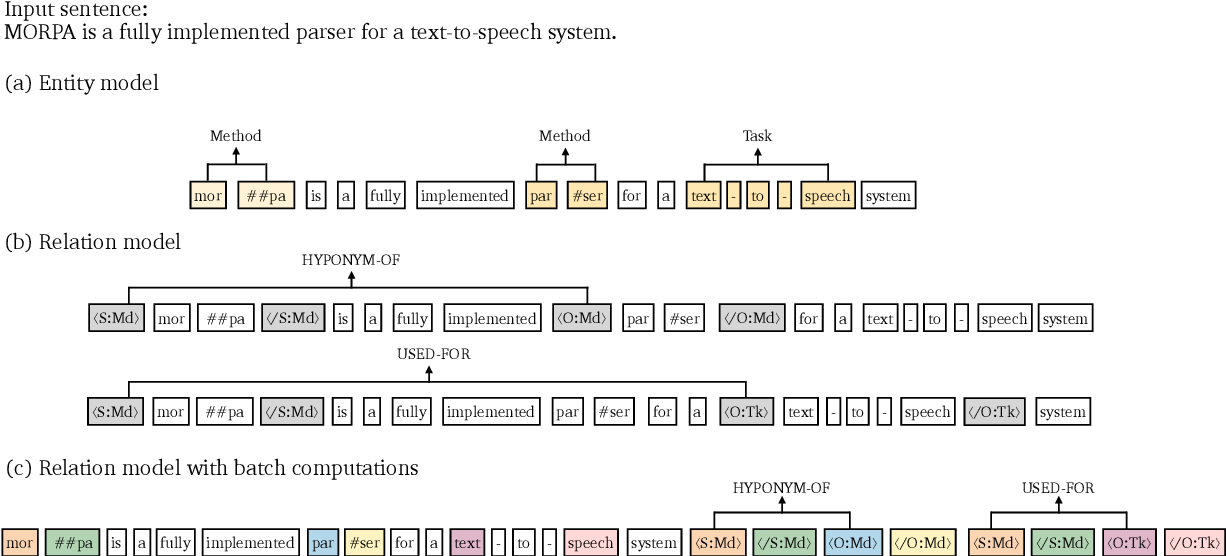
\includegraphics[width=1\textwidth]{figures/figure1.png}
    \caption{An example from the SciERC dataset Luan et al. \cite{luan-etal-2019-general}}
    \label{fig:examplefromsciercdataset}
\end{figure}

Instead, Zhong et al. \cite{Zhong2020AFE} relation model processes each pair of spans independently and inserts typed markers at the input layer to highlight the subject and object and their types. Specifically, given an input sentence \(X\) and a pair of subject-object spans \(s_i\) , \(s_j\) , where \(s_i\) , \(s_j\) have a type of \(ei , ej \in E \cup {\epsilon}\) respectively. They define text markers as \(\langle S:e_i\rangle\), \(\langle /S:e_i\rangle\), \(\langle O:e_j\rangle\), and \(\langle /O:e_j\rangle\), and insert them into the input sentence before and after the subject and object spans (Figure 1 (b)). Let \(\widehat{X}\) denote this modified sequence with text markers inserted: \(\widehat{X} = ...\langle S:e_i\rangle,x_{START(i)},...,x_{END(i)},\langle /S:e_i\rangle\,...\langle /O:e_j\rangle,x_{START(j)},...,x_{END(j)}\langle /O:e_j\rangle\)

Next, a second pre-trained encoder is applied on \(\widehat{X}\) and the output representations are denoted by \(\widehat{x}_t\). The output representations of two start positions are concatenated and the span-pair representation obtained: \[h_r(s_i,s_j)=[{\widehat{x}}_{\widehat{START(i)}};{\widehat{x}}_{\widehat{START(j)}}]\]
where \(\widehat{START(i)}\) and \(\widehat{START(j)}\) are the indices of \(\langle S:e_i\rangle\) and \(\langle O:e_j\rangle\) in \(\widehat{X}\). Finally, the representation \(h_r(s_i,s_j)\) will be fed into a feedforward network to predict the probability distribution of the relation type \(r \in R \cup {\epsilon}: P_r(r|s_i , s_j )\).

This idea of using additional markers to highlight the subject and object is not entirely new as it has been studied recently concerning classification (Zhang et al.\cite{zhang-etal-2019-ernie}; Soares et al.\cite{baldini-soares-etal-2019-matching}; Peters et al.\cite{peters2019knowledge}). However, most relation classification tasks (e.g., TACRED (Zhang et al.\cite{zhang-etal-2017-position})) only focus on a given pair of subject and object in an input sentence and its effectiveness has not been evaluated in the end-to-end setting in which Zhong et al. \cite{Zhong2020AFE} aim to classify the relationships between multiple entity mentions. They observed a large improvement in their experiments and this strengthens the hypothesis that modeling the relationship between different entity pairs in one sentence require different contextual representations. Furthermore, Zhang et al.\cite{zhang-etal-2019-ernie}; Soares et al.\cite{baldini-soares-etal-2019-matching} only consider untyped markers (e.g., \(\langle S:\rangle\), \(\langle /S:\rangle\)) and previous end-to-end models (e.g., (Wadden et al.\cite{Wadden2019EntityRA})) only inject the entity type information into the relation model through auxiliary losses. Zhong et al. \cite{Zhong2020AFE} found that injecting type information at the input layer is very helpful in distinguishing entity types — for example, whether “Disney” refers to a person or an organization— before trying to understand the relations.

